\chapter{IoT Gateway}\label{chap:iotgateway}

Unser Internet of Things Gateway besteht wiederum aus mehreren Teilen. Die einzelnen Sensoren werden entweder über den CAN-Bus oder an ein Sming angeschlossen. Der CAN-Bus wird von uns über ein BeagleBone Cape mitgelesen. Die Daten des Smings können wir ebenfalls auf dem BeagleBone empfangen. Dies erreichen wir mit Hilfe des Bluetooth Smart USB Dongle BLED112 von Bluegiga, welcher am BeagleBone angeschlossen wird.

\begin{figure}[hbtp]
    \center
    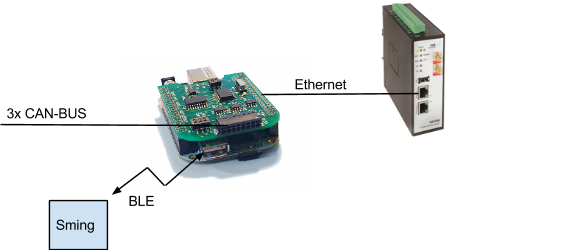
\includegraphics[width=\textwidth]{bilder/aufbau_in_auto.png}
    \caption{Aufbau des IoT Gateways}
    \label{fig:aufbau_iot_gateway}
\end{figure}


\section{SMING}\label{sec:sming}
Unsere Arbeit baut auf der Master Thesis von Daniel Meer auf. Diese wurde im Februar 2015 fertiggestellt. Daniel Meer hat diesen wie folgt beschrieben: Der TXW51 ist ein kleiner und energiesparender Sensorknoten, der als Basis für zukünftige Projekte verwendet werden kann. Er kommuniziert über Bluetooth Smart und enthält einen Sensor zur Messung der Beschleunigung. Die Firmware kann einfach für neue Anforderungen modifiziert werden.

Für unser Projekt ist vorallem die Erweiterbarkeit des Sming sehr interessant. Dies weil beliebige Senosoren über I2C angesprochen werden können, und diese beliebig im Auto verteilt werden können, ohne diese durch das diese im Auto verkabelt werden müssen.



